% !TeX spellcheck = en_GB
\subsection{Clustering 8 dimensional data}
We approached hierarchical clustering in two different ways. One consisted of simply extracting 2 of the 8 features, which we deemed most likely to give relevant and useful results, and do clustering analysis on these. Another solution was to use the feature extracting method PCA, and plot our clusters in the two first latent dimensions. Alternatively auto-encoding could have been used to reduce dimensionality but this was out of scope for this report.
\subsection{Clustering of 2 features}
The features "Property values per inhabitant" (\textbf{PV}) and "Share of 25-64 year-olds with tertiary eduction" (\textbf{TE}) were used as we suspected these would be strongly negatively correlated with the feature we have focused on in earlier reports, namely Reported thefts/burglaries per 1,000 inhabitants) (\textbf{RT}). Initially clustering was applied on the entire dataset and a target class was created based on whether the \textbf{RT} was above or below mean. However, because of the influence of time on the data, we also picked out data from a single year, 2010, which turned out to produce clearly separated clusters.
\begin{figure}[H]
	\centering
	\textbf{Hierarchical clustering with different data and linkage functions}\par\medskip
	\begin{minipage}{.5\textwidth}
		\centering
		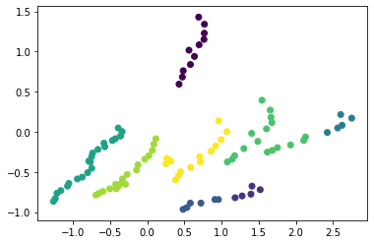
\includegraphics[width=\linewidth]{Cluster_no_class}
		\captionof{figure}{Single linkage with 2010 data}
		\label{fig:test1}
	\end{minipage}%
	\begin{minipage}{.5\textwidth}
		\centering
		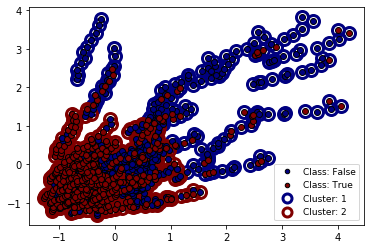
\includegraphics[width=\linewidth]{full_cluster}
		\captionof{figure}{Ward linkage with full data with target classes}
		\label{fig:test2}
	\end{minipage}
\end{figure}
\begin{figure}[H]
	\centering
	\textbf{Dendrograms based on clustering}\par\medskip
	\begin{minipage}{.5\textwidth}
		\centering
		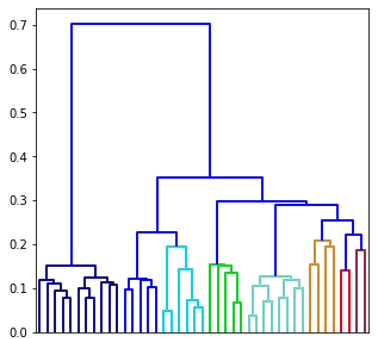
\includegraphics[width= .8\linewidth,]{Dendro_8_color}
		\captionof{figure}{Dendrogram for single linkage on 2010 data}
		\label{fig:test1}
	\end{minipage}%
	\begin{minipage}{.5\textwidth}
		\centering
		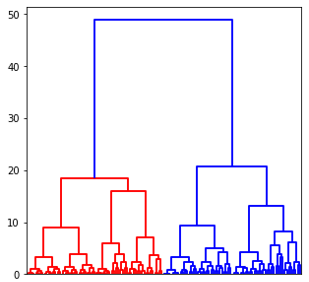
\includegraphics[width= .8\linewidth]{dendro_full_color}
		\captionof{figure}{Dendrogram for ward linkage on full data}
		\label{fig:test2}
	\end{minipage}
\end{figure}
\noindent
Though the similarity measure remained the same, namely euclidean distance, the linkage functions were changed to fit the data better.
As seen in Figure 2.2, the data from 2010, was separated clearly in quite straight lines, and therefore single linkage clustering seemed appropriate.
Single linkage is done by repeatedly clustering together the two closest clusters, when initializing every data point as a cluster, until the correct number of clusters is reached. This distance between two clusters $C_1$ and $C_2$, is then described by:
\begin{equation}
	d(C_1,C_2) = \underset{\mathbf x \in C_1, \mathbf y \in C_2}{\min} \len{\mathbf x-\mathbf y}
\end{equation}
In choosing the number of clusters, we simply counted the number of straight lines in the plot, which worked well.
In the full dataset the clusters were not as easy to distinguish between, but it was obvious that the linear nature of the data was consistent over many years.
As the target feature was binary, we choose 2 clusters for the full dataset and the Ward linkage was used.
Ward linkage is a center-based clustering method, that connects clusters based on the least squared error between the points and the centroid in a cluster. This method is inspired by the $K$-means algorithm, the precise mathematical description of which can be read in [1] (p. 297).
%\begin{equation}
%	\sum_{i = 1 }^N \sum_{k = 1 }^K z_{ik} || x_i - \mu_k ||^2_2 
%\end{equation}
As the data seemed to emanate in linear fashion from a small area around (-1.5,-1.5) we also attempted to parallel shift the data by 1.5 on each axis and use the similarity measure, cosine, as this could encapsulate the circular quality of the data. This, however, did not yield better results, and was discarded.
\subsection{Cluster types}
In \cite{skynet1} we performed PCA.
We plotted the observations in the first two latent dimensions, as shown on figure \ref{fig:PCA}.
\begin{figure}[H]
	\centering
	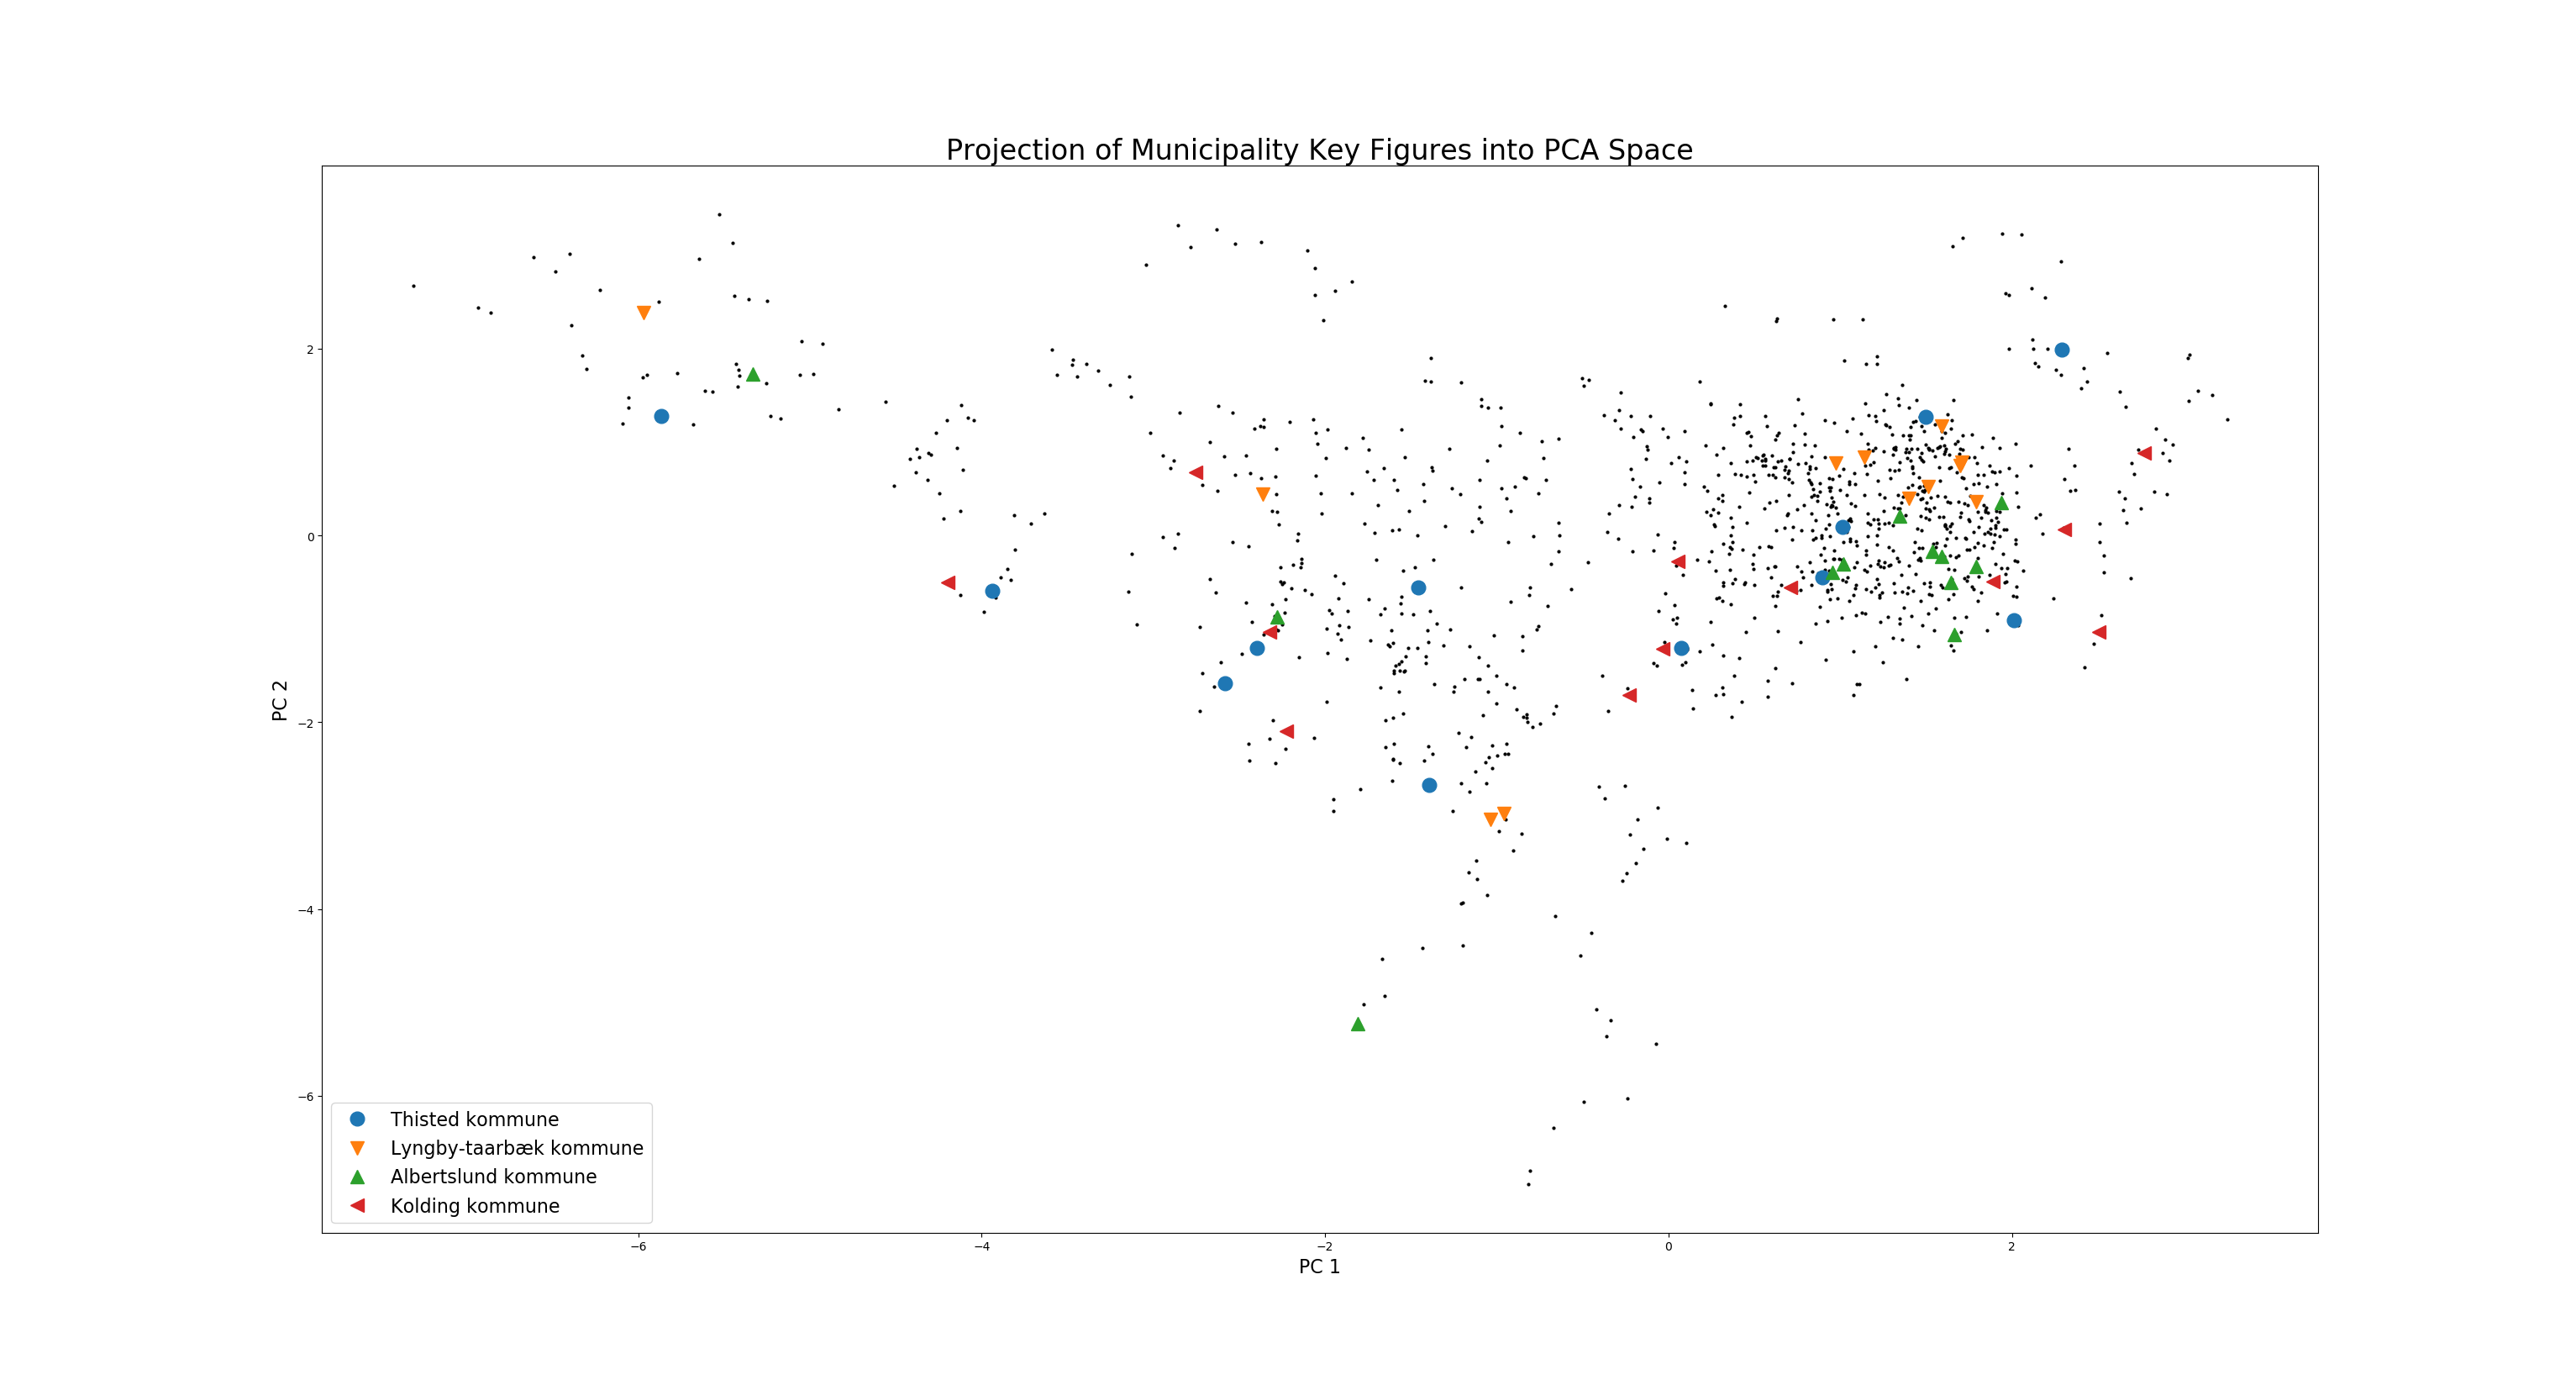
\includegraphics[width=.7\textwidth]{pca}
	\caption{The first two principal components of the dataset.}\label{fig:PCA}
\end{figure}\noindent
Figure \ref{fig:PCA} shows only the first two principal components, so some information is lost.
However, there does seem to be some clusters, even though they are rather ill-defined.
They seem to be mainly center-based, such that most points are closer to the center of their respective clusters than any other cluster centers.
This is of course not true for every point and depends on where the real clusters are, however it still gives an idea of the structure of the dataset.

\subsection{Clusting be Gaussian Mixture Model(GMM)}
As mentioned earlier, the target data was transformed into a binary set of classes depending on whether the \textbf{RT} feature was below or above mean. As such, there only existed two true labels, here named \textit{Low Risk} and \textit{High Risk}. Therefore we started out by training a Gaussian Mixture Model (GMM) with K=2 clusters using the \textit{sklearn} python library. In \textit{sklearn} the GMM implements the expectation-maximization(EM) algorithm to do the fitting of the mixture Gaussian model to get the parameters for $\mu$ (mean), $\Sigma$ (covariance matrix), and $\pi$ (weights) that best approximate the dataset.
\\
As K was set to 2 we instead made the covariance type (cv-type) the variable and created a couple of experiments just to get an idea of how the cv-type can influence accuracy when predicting clusters for the two classes of data points. Four cv-types were investigated
\begin{table}[H]
	\centering
	\begin{tabular}{|l|l|}
		\hline
		\textbf{Cv-type} & \textbf{Description} \\
		\hline
		Full & Each component has its own general covariance matrix\\
		Tied & All components share the same general covariance matrix\\
		Diag & Each component has its own diagonal covariance matrix\\
		Spherical & Each component has its own single variance\\
		\hline
	\end{tabular}
\end{table}
\noindent
\begin{figure}[H]
	\centering
	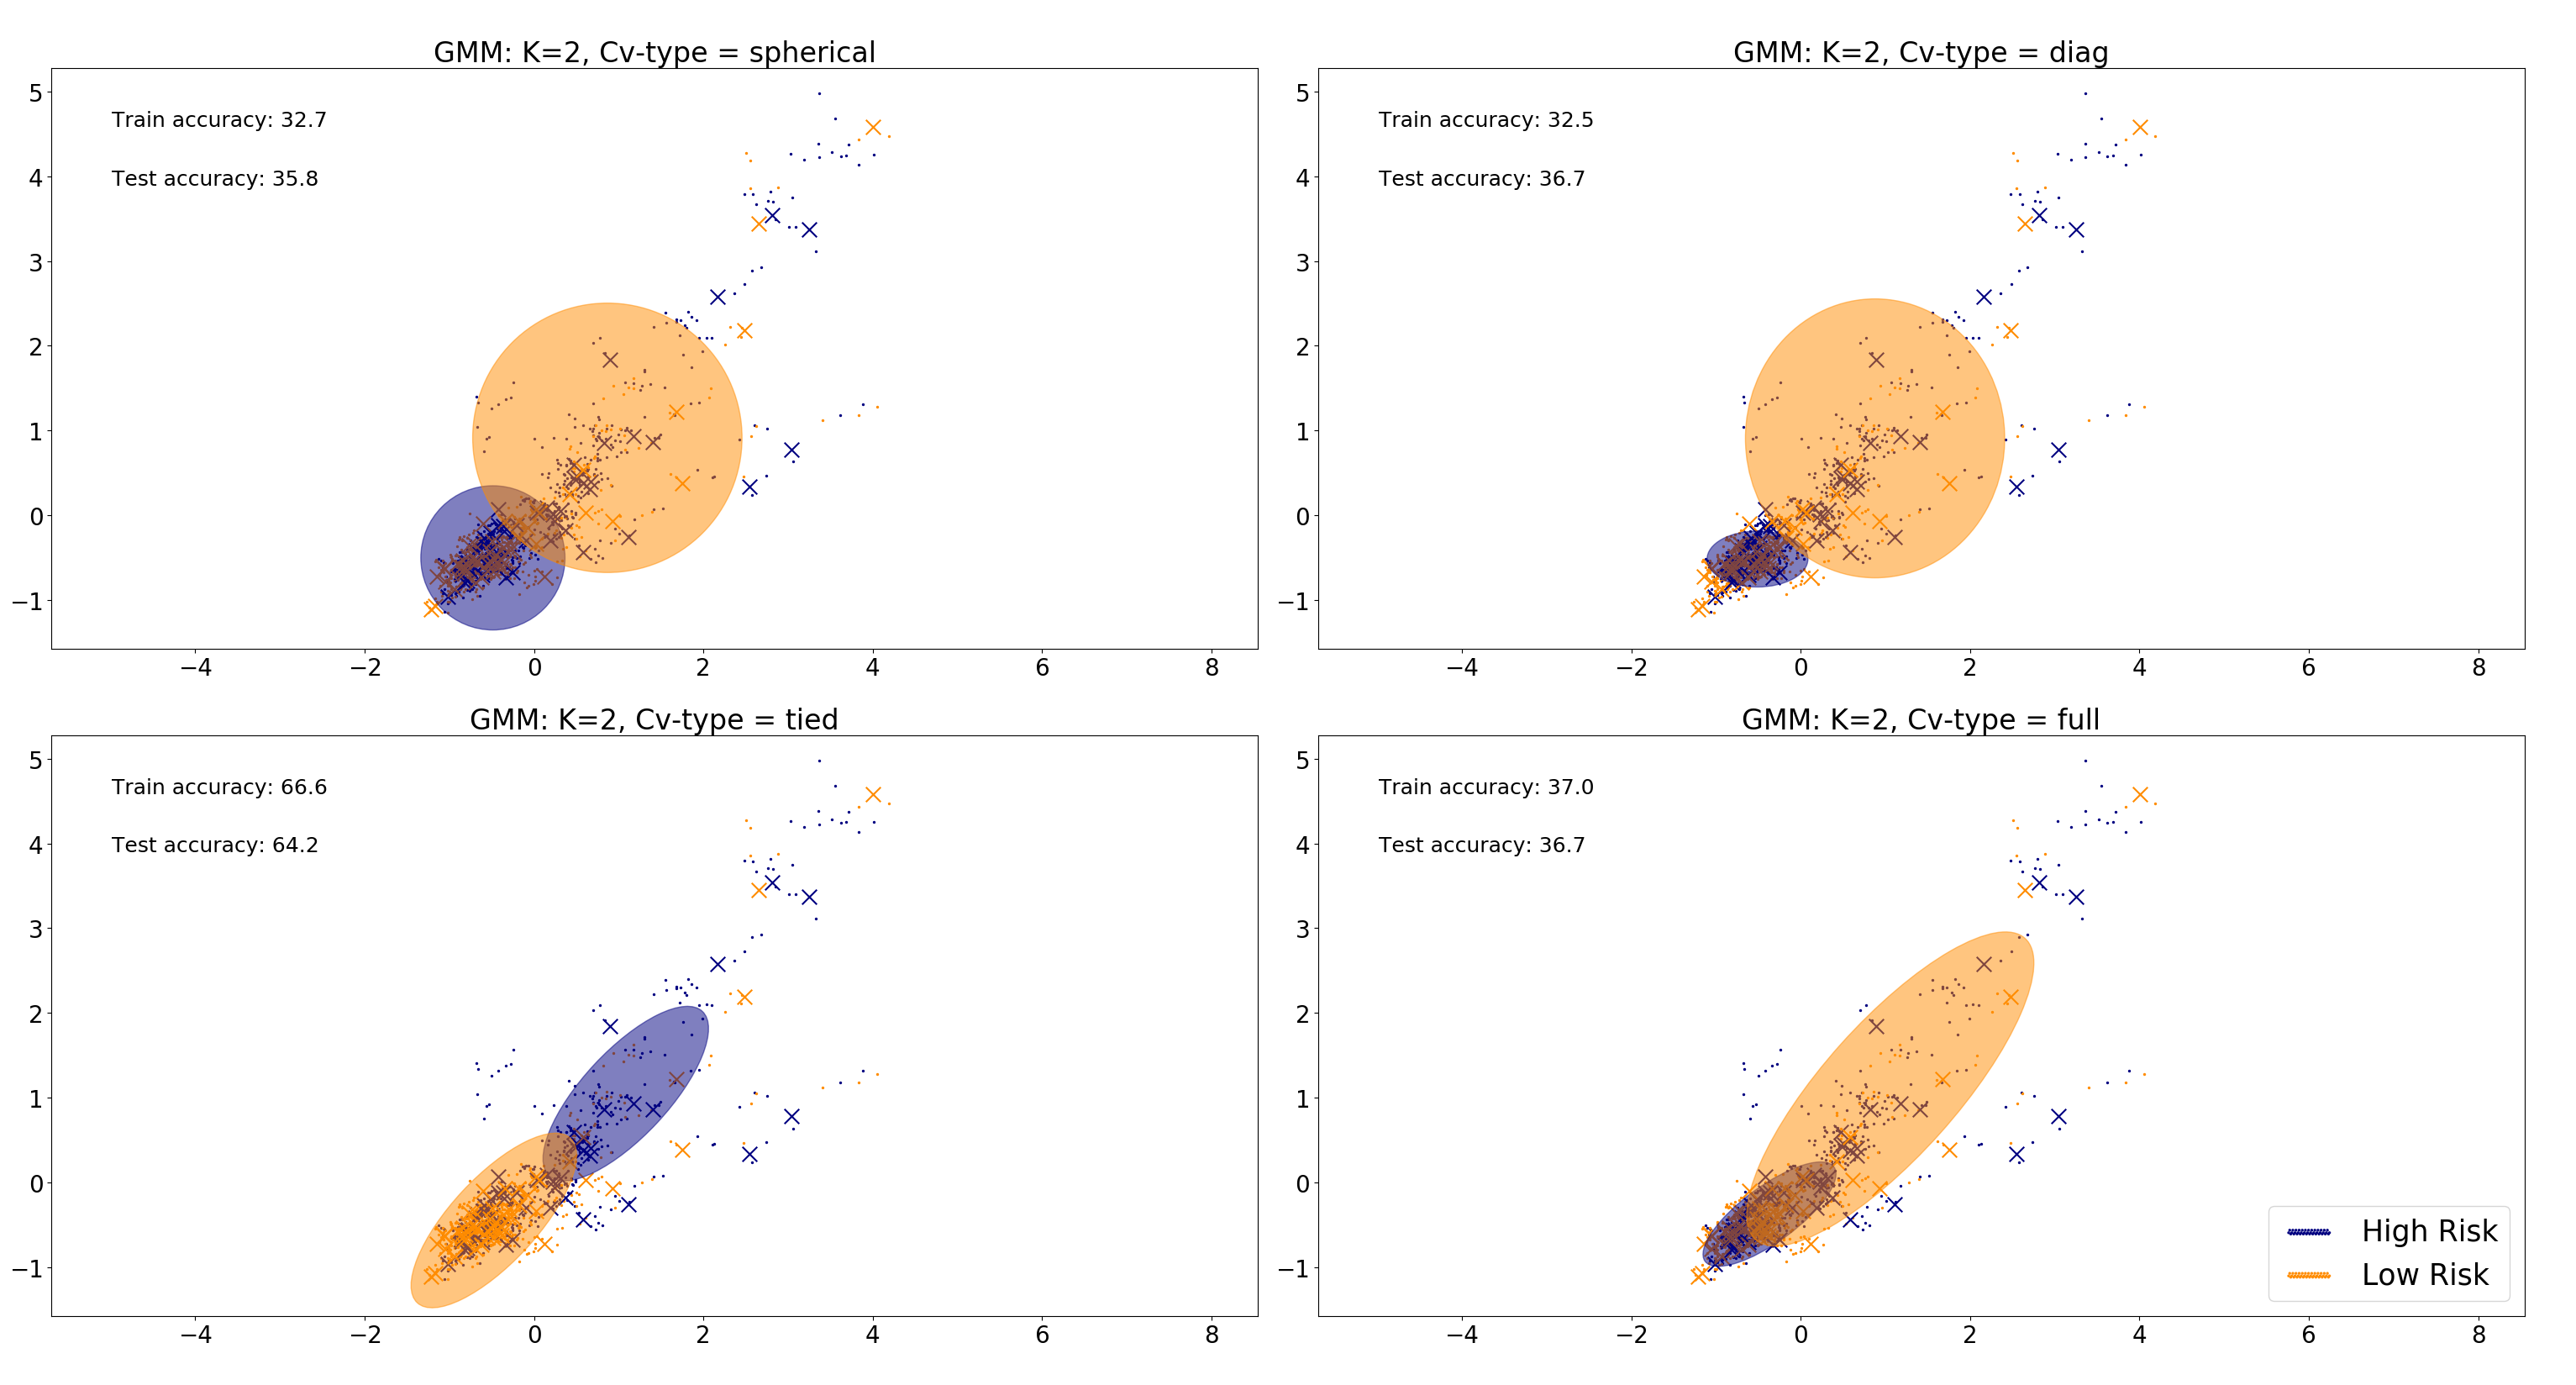
\includegraphics[width=\textwidth]{accuracy_GMM}
	\caption{Accuracy of GMM, in a single fold, based on covariance type. Test data is plotted with an 'X'}\label{fig:PCA}
\end{figure}\noindent
From the result it was possible to get an idea about the cv-type and its influence on the clustering. From the results it looked like the \textit{tied} cv-type might be worth looking into. But, this was just based on a few experiments on a couple of training and test folds, not an entire cross-validation. As mentioned earlier, these experiments were only performed to enhance our understanding of the co-variance type. To be able to actually rely on the results a thorough validation should be performed, which has not been pursued in this report. But, nonetheless the experiments points in a direction of the \textit{tied} cv-type being worth looking into for this clustering problem.
\\
Besides testing the data on two predefined clusters, we thought it interesting to investigate which number of cluster components would be chosen as the best fit for the data. For this a two-layer cross validation was used on GMMs with cv-type \textit{full} and $ K=1 $ to $ K=30 $ cluster components. The cv-type \textit{full} was used due to issues with the matrix shape when trying out the \textit{tied} cv-type.
The score of the fit was made using the negative log-likelihood
\begin{equation}
\begin{aligned} -\mathcal{L}^{\text {test }}(\boldsymbol{\pi}, \boldsymbol{\mu}, \boldsymbol{\Sigma}) &= -\log p\left(\boldsymbol{X}^{\text {test }} | \boldsymbol{\mu}, \boldsymbol{\Sigma}, \boldsymbol{\pi}\right) \\ &= -\sum_{i=1}^{N^{\text {test }}} \log \left[\sum_{k=1}^{K} \pi_{k} \mathcal{N}\left(\boldsymbol{x}_{i}^{\text {test }} | \boldsymbol{\mu}_{k}, \boldsymbol{\Sigma}_{k}\right)\right] \end{aligned}
\end{equation}
which can be computed using the negative result of the sum of the \textit{sklearn} function \textit{score\_samples} from the \textit{GaussianMixture} class.
\\
The cross-validation resulted in K=14 as the optimal number of clusters for lowering the negative log-likelihood. The resulting clusters are illustrated in the figure below.
\begin{figure}[H]
	\centering
	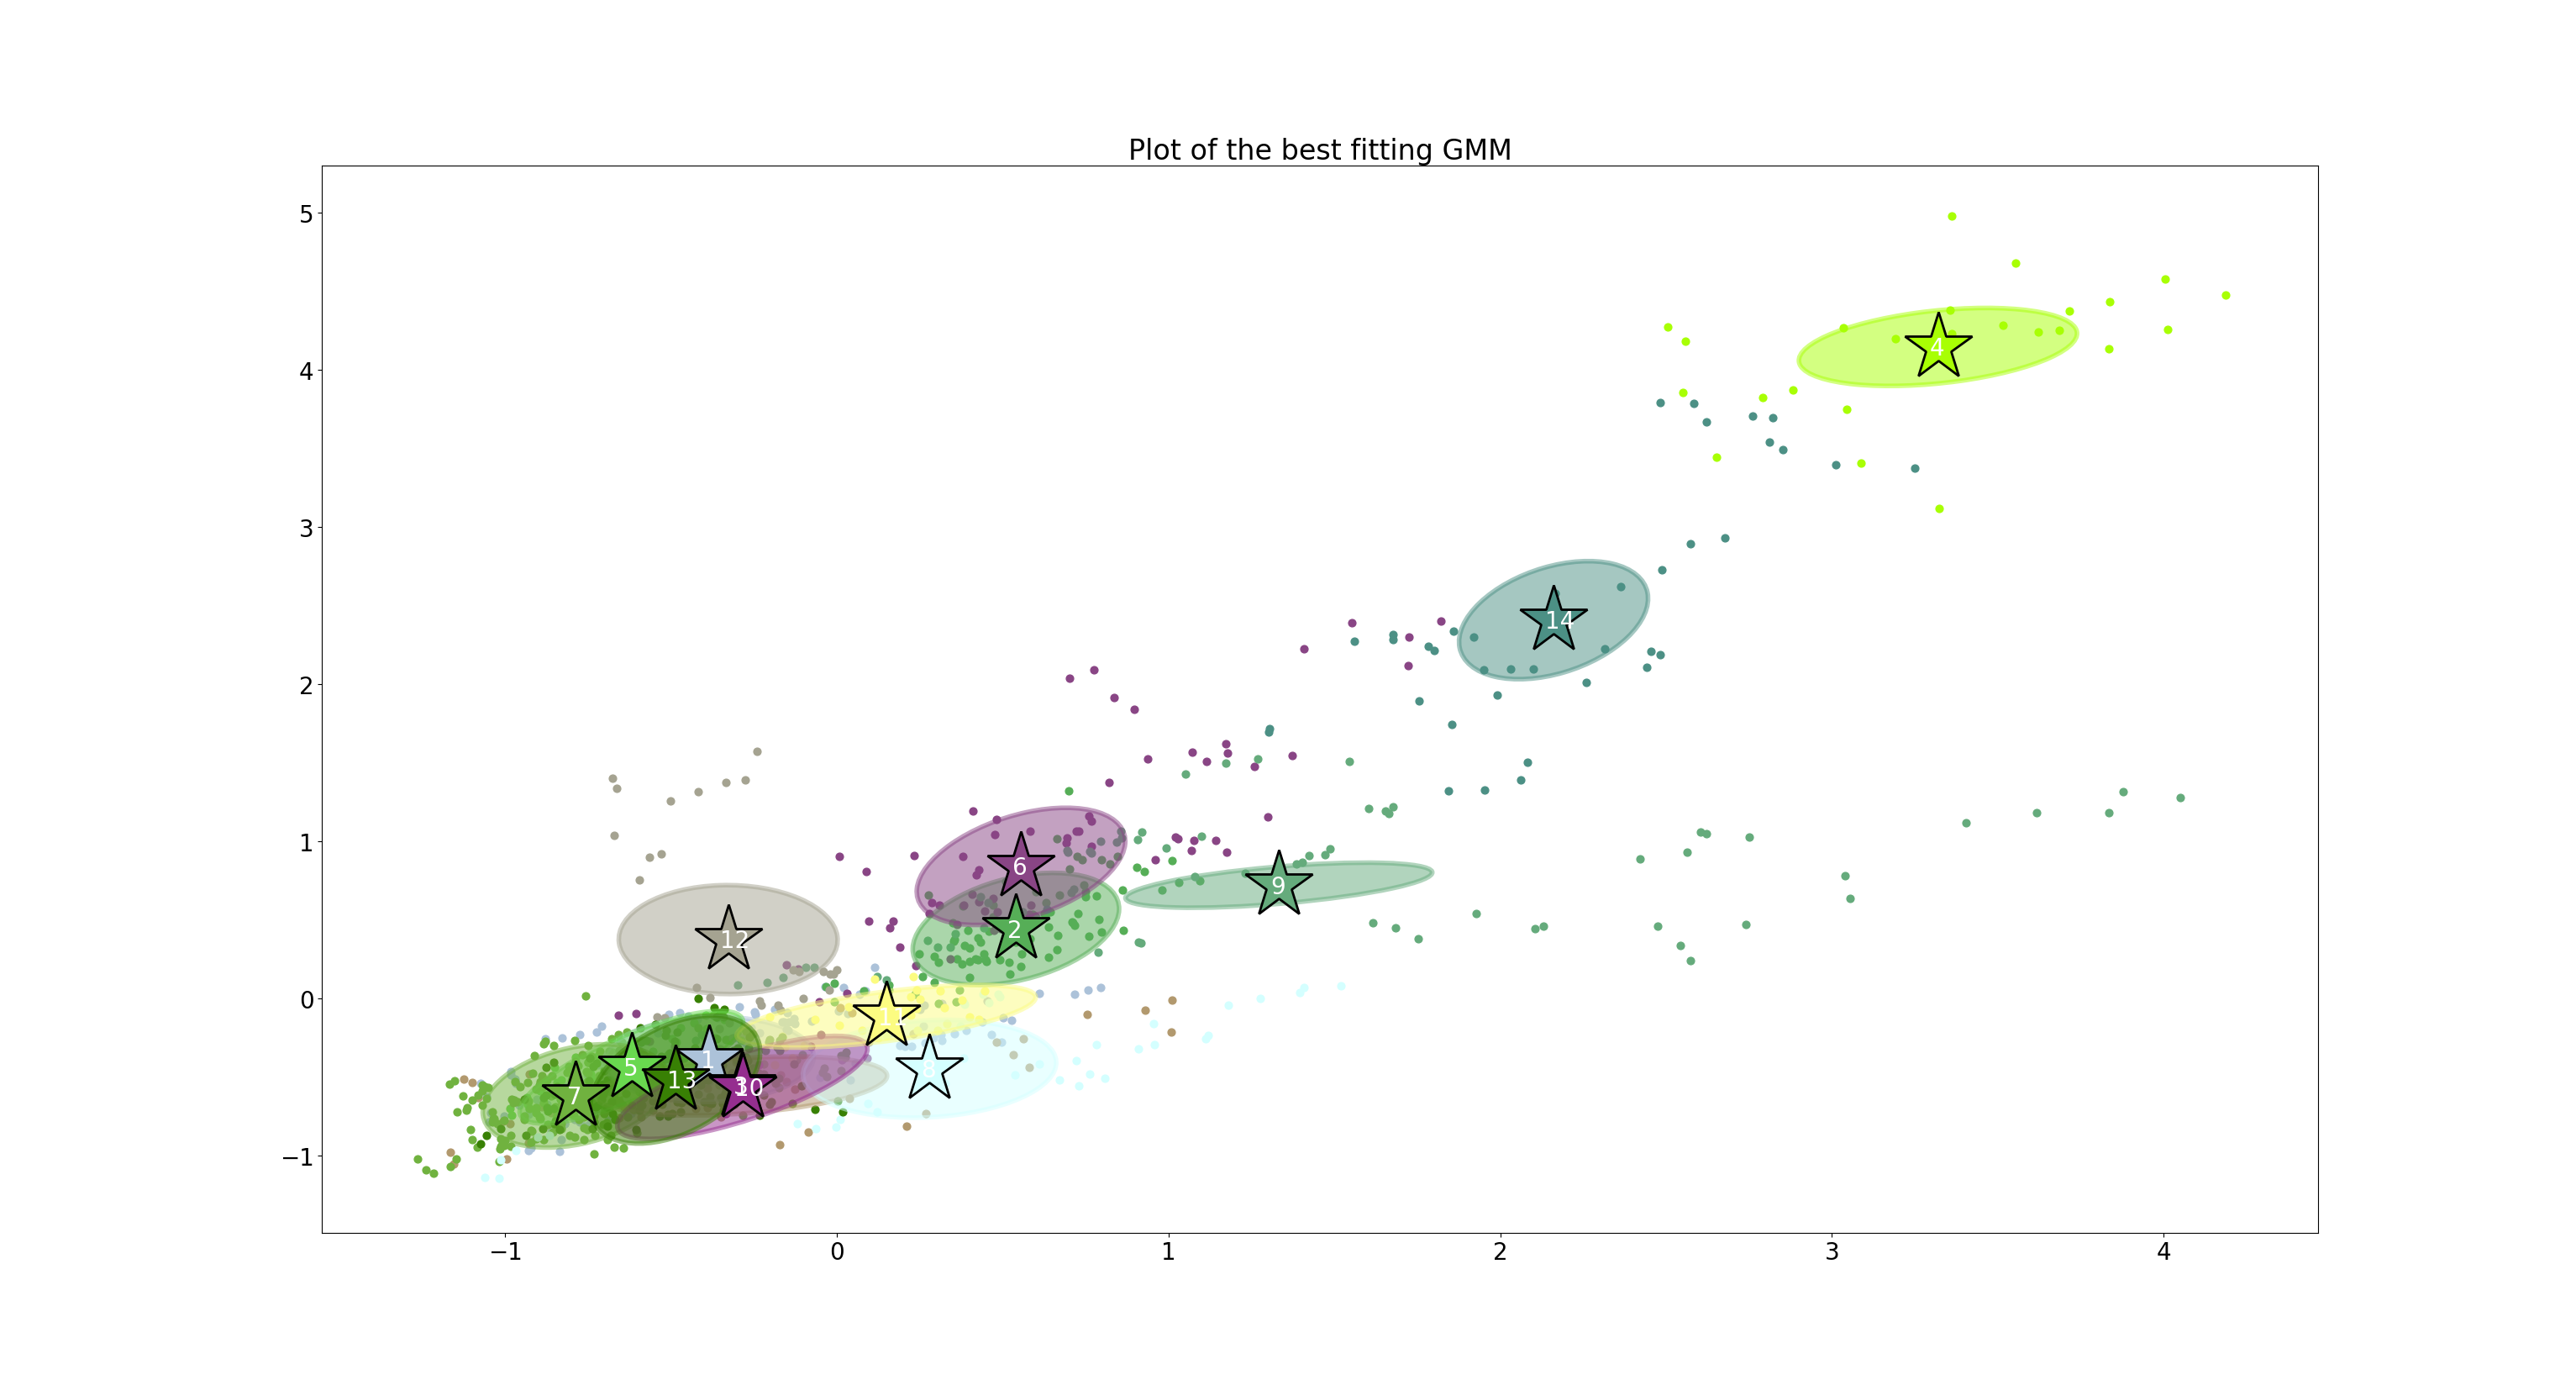
\includegraphics[width=\textwidth]{best_fitting_GMM}
	\caption{The winning GMM from nested cross validation with $ K=14 $ clusters}\label{fig:PCA}
\end{figure}\noindent
The ellipses for each Gaussian component was drawn in the eigenvector space and normalized to avoid the clusters painting over the entire plot and the data point were assigned the color of the cluster component to which they belong. The stars show the centroids of each cluster and the numbering, even though a bit off, serves the purpose of referencing the clusters in this report. Looking at the plot lower left corner, the clusters overlap a lot and end up being one big clutter. This makes it difficult to judge whether or not the clusters actually makes sense and therefore one should be careful of just accepting the GMM as a good fit for the data. On the other hand cluster 2, 6, and 9 around the middle and cluster 4, and 14 in the top right corner seems quite plausible in the way they fit the data. So from the plot it looks like 14 clusters might be a bit too many, but still there is probably a lot more groupings in the data than just the two we created in this experiment.

\subsection{Quality testing the GMM}
Now looking at the quality of the GMM according to the binary classes, we tried both a model with two clusters and the optimal with 14, just for fun. We expected the model with 14 clusters to do a very poor job, since the many classes did not match the two classes created by us. Surely, the results were bad, which can be seen in the table below:

\begin{table}[H]
	\centering
	\begin{tabular}{|l|l|}
		\hline
		\textbf{Quality Test Type} & \textbf{Score} \\
		\hline
		Rand Index Score & 0.5125658265331962\\
		Jaccard Similarity Score & 0.11132711900604264\\
		Normalized Mutual Information (NMI) Score & 0.08118995950534755\\
		\hline
	\end{tabular}
\end{table}
\noindent
The rand index score shows a similarity of approximately 51 percent, so the 14 cluster GMM only agrees with the true labels about half the time. Also, a problem that we need to be aware of here is, that when there are a lot of clusters, as in this experiment, the Rand index has a tendency to be artificially close to 1 (completely similar). This is something the Jaccard similarity score tries to avoid. And as it turns out, this score shows a lot less similarity, only about 11 percent, which is a bit more realistic. Finally the NMI tries to quantify how much information the partition provides about the other. And here we hit a bottom low with only 8 percent similarity. After all this was expected as explained earlier. We then thought it interesting to see how a $ K=2 $ GMM would perform on the data.
We tried to test it and got the following result:
\begin{figure}[H]
	\centering
	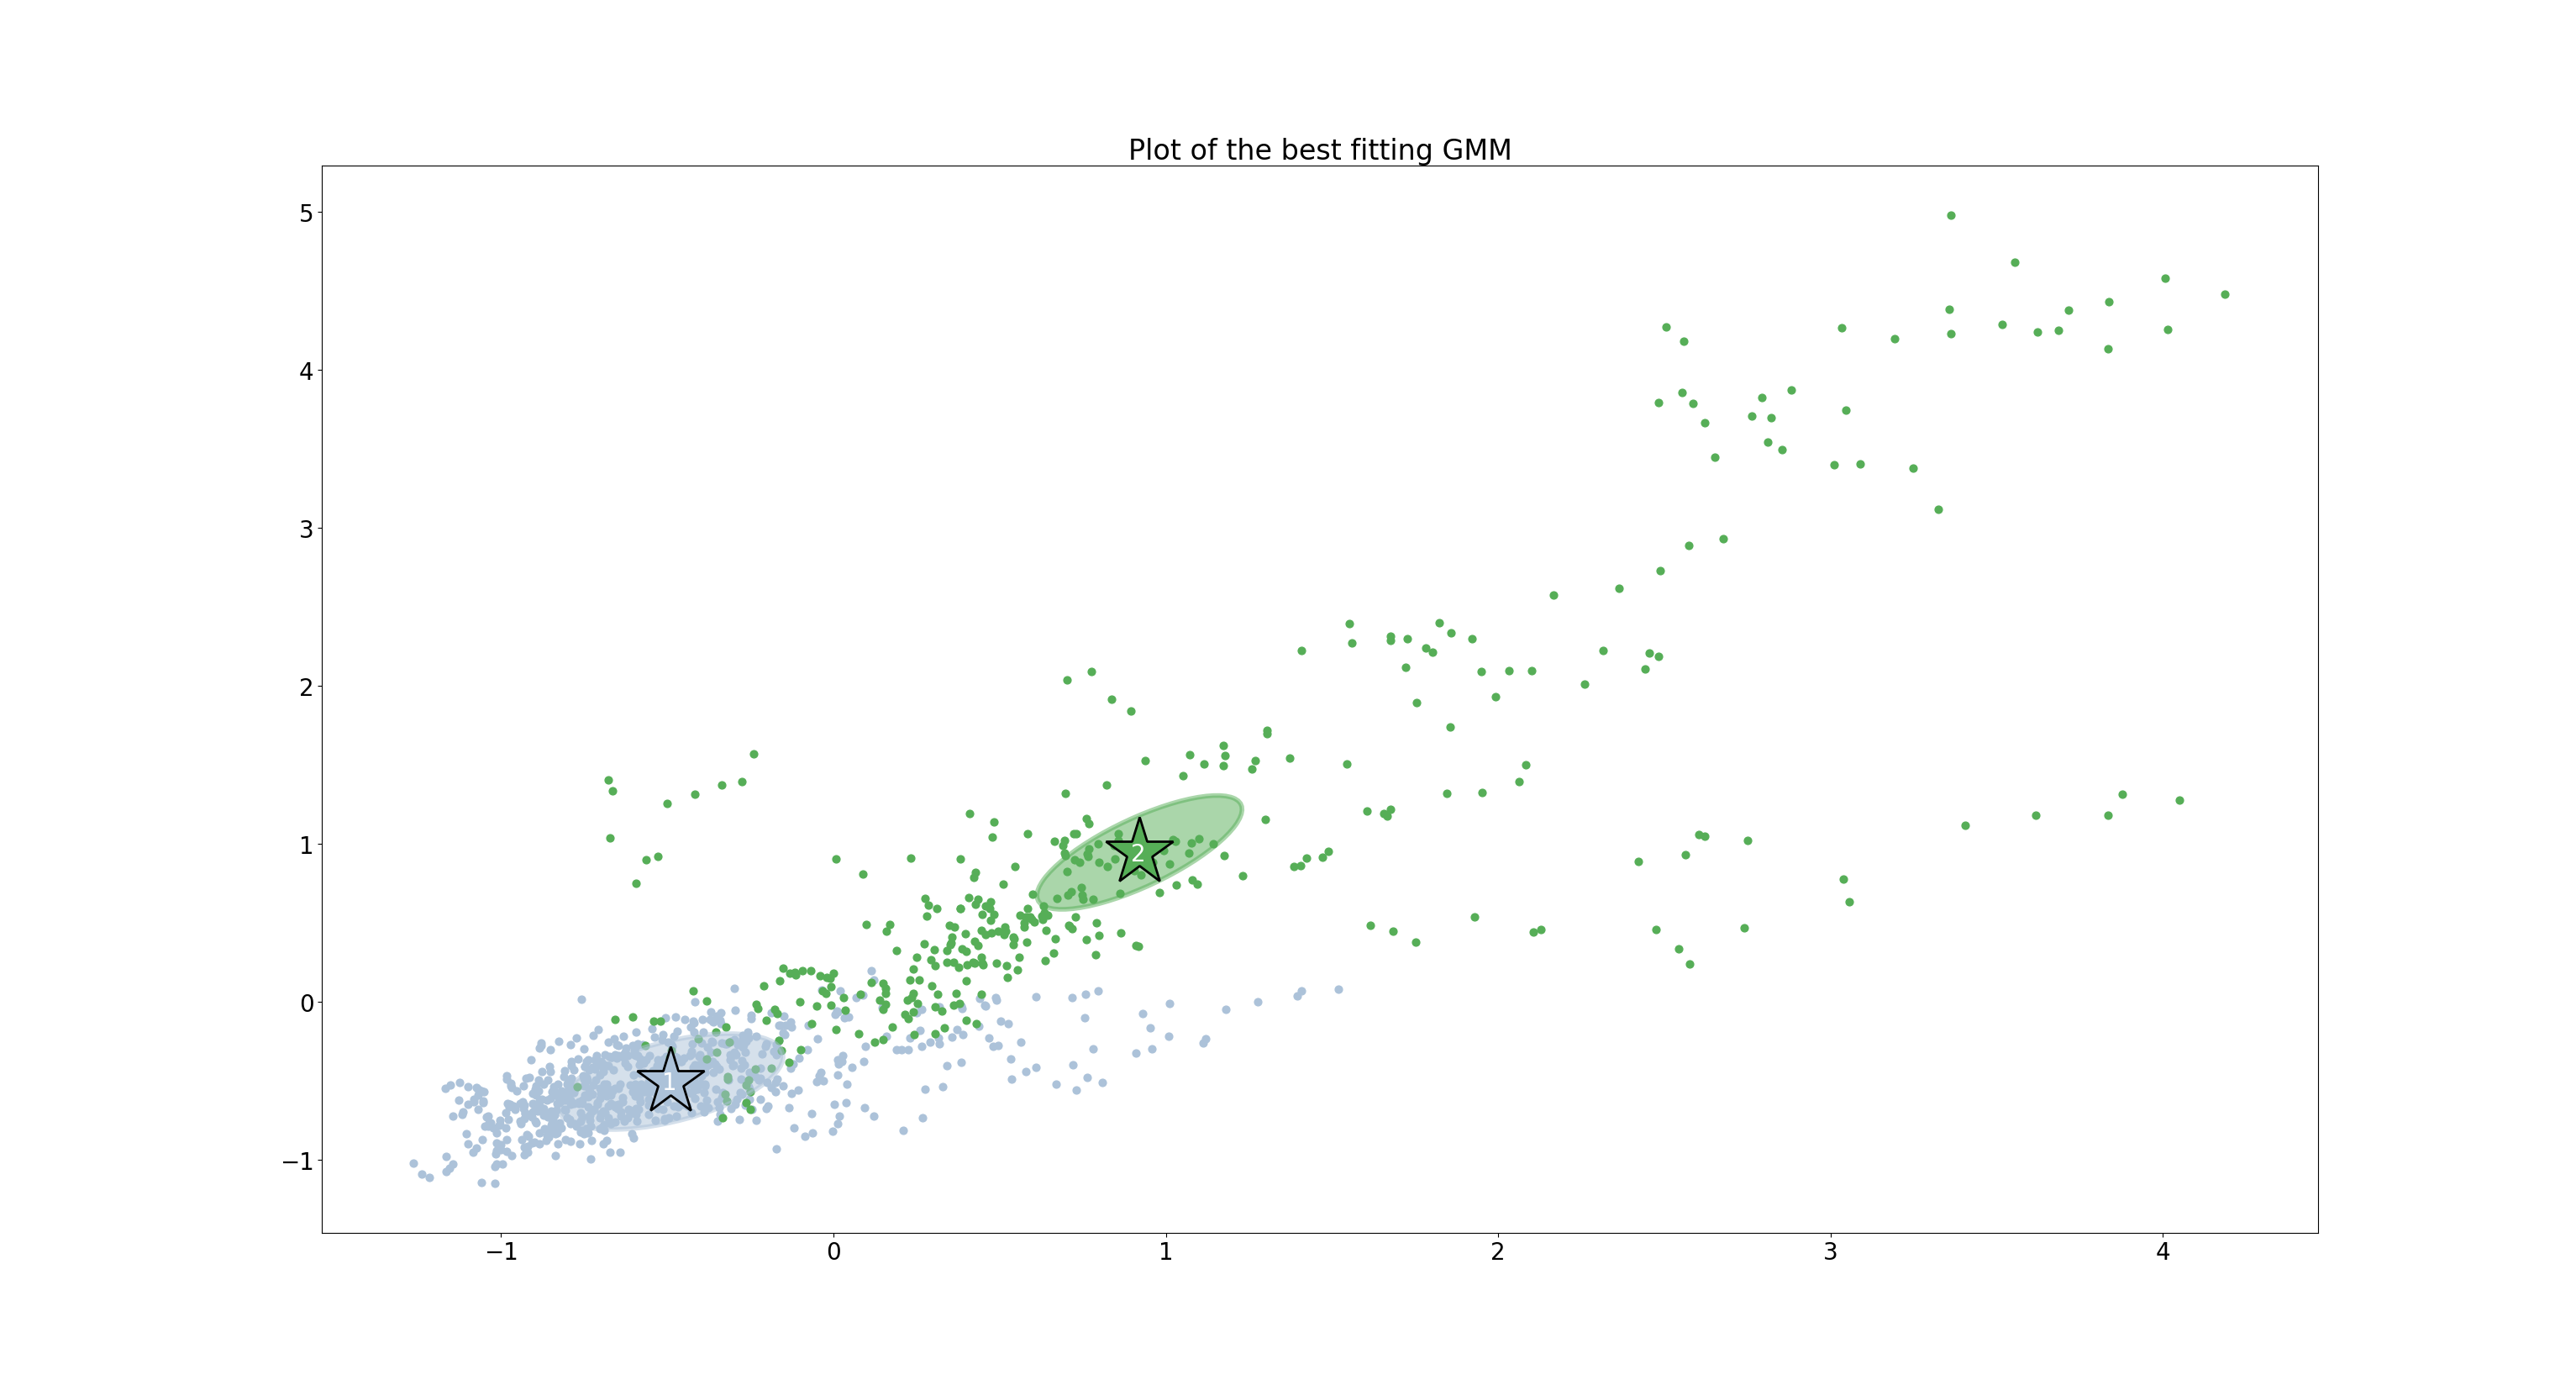
\includegraphics[width=\textwidth]{GMM_2_clusters}
	\caption{GMM $ K=2 $ clustering}\label{fig:PCA}
\end{figure}\noindent
interestingly enough the similarity scores were not that different here:
\begin{table}[H]
	\centering
	\begin{tabular}{|l|l|}
		\hline
		\textbf{Quality Test Type} & \textbf{Score} \\
		\hline
		Rand Index Score & 0.5630392952318937\\
		Jaccard Similarity Score & 0.2112678802282913\\
		Normalized Mutual Information(NMI) Score & 0.11482413218698861\\
		\hline
	\end{tabular}
\end{table}
\noindent
This all in all points to the conclusion, that the settings for the GMM might not fit that data very well, and that further experiments for tuning other parameters like the regularization constant $\lambda$ or the cv-type should be conduct. Also, it could be an option simply to try other models for the data than a GMM.